% Options for packages loaded elsewhere
\PassOptionsToPackage{unicode}{hyperref}
\PassOptionsToPackage{hyphens}{url}
\PassOptionsToPackage{dvipsnames,svgnames,x11names}{xcolor}
%
\documentclass[
]{scrartcl}
\usepackage{amsmath,amssymb}
\usepackage{lmodern}
\usepackage{iftex}
\ifPDFTeX
  \usepackage[T1]{fontenc}
  \usepackage[utf8]{inputenc}
  \usepackage{textcomp} % provide euro and other symbols
\else % if luatex or xetex
  \usepackage{unicode-math}
  \defaultfontfeatures{Scale=MatchLowercase}
  \defaultfontfeatures[\rmfamily]{Ligatures=TeX,Scale=1}
\fi
% Use upquote if available, for straight quotes in verbatim environments
\IfFileExists{upquote.sty}{\usepackage{upquote}}{}
\IfFileExists{microtype.sty}{% use microtype if available
  \usepackage[]{microtype}
  \UseMicrotypeSet[protrusion]{basicmath} % disable protrusion for tt fonts
}{}
\makeatletter
\@ifundefined{KOMAClassName}{% if non-KOMA class
  \IfFileExists{parskip.sty}{%
    \usepackage{parskip}
  }{% else
    \setlength{\parindent}{0pt}
    \setlength{\parskip}{6pt plus 2pt minus 1pt}}
}{% if KOMA class
  \KOMAoptions{parskip=half}}
\makeatother
\usepackage{xcolor}
\usepackage[a4paper,width=160mm,top=35mm,bottom=30mm,bindingoffset=0mm]{geometry}
\usepackage{color}
\usepackage{fancyvrb}
\newcommand{\VerbBar}{|}
\newcommand{\VERB}{\Verb[commandchars=\\\{\}]}
\DefineVerbatimEnvironment{Highlighting}{Verbatim}{commandchars=\\\{\}}
% Add ',fontsize=\small' for more characters per line
\usepackage{framed}
\definecolor{shadecolor}{RGB}{248,248,248}
\newenvironment{Shaded}{\begin{snugshade}}{\end{snugshade}}
\newcommand{\AlertTok}[1]{\textcolor[rgb]{0.94,0.16,0.16}{#1}}
\newcommand{\AnnotationTok}[1]{\textcolor[rgb]{0.56,0.35,0.01}{\textbf{\textit{#1}}}}
\newcommand{\AttributeTok}[1]{\textcolor[rgb]{0.77,0.63,0.00}{#1}}
\newcommand{\BaseNTok}[1]{\textcolor[rgb]{0.00,0.00,0.81}{#1}}
\newcommand{\BuiltInTok}[1]{#1}
\newcommand{\CharTok}[1]{\textcolor[rgb]{0.31,0.60,0.02}{#1}}
\newcommand{\CommentTok}[1]{\textcolor[rgb]{0.56,0.35,0.01}{\textit{#1}}}
\newcommand{\CommentVarTok}[1]{\textcolor[rgb]{0.56,0.35,0.01}{\textbf{\textit{#1}}}}
\newcommand{\ConstantTok}[1]{\textcolor[rgb]{0.00,0.00,0.00}{#1}}
\newcommand{\ControlFlowTok}[1]{\textcolor[rgb]{0.13,0.29,0.53}{\textbf{#1}}}
\newcommand{\DataTypeTok}[1]{\textcolor[rgb]{0.13,0.29,0.53}{#1}}
\newcommand{\DecValTok}[1]{\textcolor[rgb]{0.00,0.00,0.81}{#1}}
\newcommand{\DocumentationTok}[1]{\textcolor[rgb]{0.56,0.35,0.01}{\textbf{\textit{#1}}}}
\newcommand{\ErrorTok}[1]{\textcolor[rgb]{0.64,0.00,0.00}{\textbf{#1}}}
\newcommand{\ExtensionTok}[1]{#1}
\newcommand{\FloatTok}[1]{\textcolor[rgb]{0.00,0.00,0.81}{#1}}
\newcommand{\FunctionTok}[1]{\textcolor[rgb]{0.00,0.00,0.00}{#1}}
\newcommand{\ImportTok}[1]{#1}
\newcommand{\InformationTok}[1]{\textcolor[rgb]{0.56,0.35,0.01}{\textbf{\textit{#1}}}}
\newcommand{\KeywordTok}[1]{\textcolor[rgb]{0.13,0.29,0.53}{\textbf{#1}}}
\newcommand{\NormalTok}[1]{#1}
\newcommand{\OperatorTok}[1]{\textcolor[rgb]{0.81,0.36,0.00}{\textbf{#1}}}
\newcommand{\OtherTok}[1]{\textcolor[rgb]{0.56,0.35,0.01}{#1}}
\newcommand{\PreprocessorTok}[1]{\textcolor[rgb]{0.56,0.35,0.01}{\textit{#1}}}
\newcommand{\RegionMarkerTok}[1]{#1}
\newcommand{\SpecialCharTok}[1]{\textcolor[rgb]{0.00,0.00,0.00}{#1}}
\newcommand{\SpecialStringTok}[1]{\textcolor[rgb]{0.31,0.60,0.02}{#1}}
\newcommand{\StringTok}[1]{\textcolor[rgb]{0.31,0.60,0.02}{#1}}
\newcommand{\VariableTok}[1]{\textcolor[rgb]{0.00,0.00,0.00}{#1}}
\newcommand{\VerbatimStringTok}[1]{\textcolor[rgb]{0.31,0.60,0.02}{#1}}
\newcommand{\WarningTok}[1]{\textcolor[rgb]{0.56,0.35,0.01}{\textbf{\textit{#1}}}}
\usepackage{longtable,booktabs,array}
\usepackage{calc} % for calculating minipage widths
% Correct order of tables after \paragraph or \subparagraph
\usepackage{etoolbox}
\makeatletter
\patchcmd\longtable{\par}{\if@noskipsec\mbox{}\fi\par}{}{}
\makeatother
% Allow footnotes in longtable head/foot
\IfFileExists{footnotehyper.sty}{\usepackage{footnotehyper}}{\usepackage{footnote}}
\makesavenoteenv{longtable}
\usepackage{graphicx}
\makeatletter
\def\maxwidth{\ifdim\Gin@nat@width>\linewidth\linewidth\else\Gin@nat@width\fi}
\def\maxheight{\ifdim\Gin@nat@height>\textheight\textheight\else\Gin@nat@height\fi}
\makeatother
% Scale images if necessary, so that they will not overflow the page
% margins by default, and it is still possible to overwrite the defaults
% using explicit options in \includegraphics[width, height, ...]{}
\setkeys{Gin}{width=\maxwidth,height=\maxheight,keepaspectratio}
% Set default figure placement to htbp
\makeatletter
\def\fps@figure{htbp}
\makeatother
\setlength{\emergencystretch}{3em} % prevent overfull lines
\providecommand{\tightlist}{%
  \setlength{\itemsep}{0pt}\setlength{\parskip}{0pt}}
\setcounter{secnumdepth}{5}
% Set your Title, name, supervisor etc.
\newcommand{\mytitle}{My Super Fancy Thesis Title}
\newcommand{\myname}{Jane Doe}
\newcommand{\mysupervisor}{Dr Dre}
\newcommand{\dueday}{dd}
\newcommand{\duemonth}{Month}
\newcommand{\dueyear}{yyyy}


% Add more specific packages, e.g.
% \usepackage{alltt}
% \usepackage{ragged2e}


% Defining fancy header -- don't touch
\usepackage{fancyhdr}
\newcommand{\changefont}{%
    \fontsize{8}{11}\selectfont
}
\pagestyle{fancy}
\fancyhead{}
\fancyhead[R]{\changefont{\mytitle}}
\fancyfoot{}
\fancyfoot[R]{\thepage}
\setlength{\headheight}{14.5pt}
\setlength{\parindent}{0pt}
\interfootnotelinepenalty = 10000
\ifLuaTeX
  \usepackage{selnolig}  % disable illegal ligatures
\fi
\usepackage[round, comma]{natbib}
\bibliographystyle{plainnat}
\IfFileExists{bookmark.sty}{\usepackage{bookmark}}{\usepackage{hyperref}}
\IfFileExists{xurl.sty}{\usepackage{xurl}}{} % add URL line breaks if available
\urlstyle{same} % disable monospaced font for URLs
\hypersetup{
  colorlinks=true,
  linkcolor={blue},
  filecolor={Maroon},
  citecolor={Blue},
  urlcolor={Blue},
  pdfcreator={LaTeX via pandoc}}

\author{}
\date{\vspace{-2.5em}}

\begin{document}

% FRONT PAGE -------------------------------------------------------------------

\begin{titlepage}
\begin{center}

\LARGE
Master's Thesis

\vspace{0.5cm}

\rule{\textwidth}{1.5pt}
\LARGE
\textbf{\mytitle}
\rule{\textwidth}{1.5pt}

\vspace{0.5cm}

\large
Department of Statistics \\
Ludwig-Maximilians-Universität München

\vfill

\Large
\textbf{\myname}

\vfill

\large
Munich, \dueday~\duemonth~\dueyear

\vfill


\includegraphics[width = 0.4\textwidth]{params/sigillum.png}

\vfill

\normalsize
Submitted in partial fulfillment of the requirements for the degree of M. Sc.
\\

Supervised by \mysupervisor

\end{center}
\end{titlepage}

\pagenumbering{roman}
\newpage

\begin{abstract}

Lorem ipsum dolor sit amet, consectetur adipiscing elit, sed do eiusmod tempor
incididunt ut labore et dolore magna aliqua. Ut enim ad minim veniam, quis
nostrud exercitation ullamco laboris nisi ut aliquip ex ea commodo consequat.
Duis aute irure dolor in reprehenderit in voluptate velit esse cillum dolore eu
fugiat nulla pariatur. Excepteur sint occaecat cupidatat non proident, sunt in
culpa qui officia deserunt mollit anim id est laborum.

\end{abstract}

\newpage

{
\hypersetup{linkcolor=}
\setcounter{tocdepth}{2}
\tableofcontents
}
\newpage
\listoffigures
\newpage

\pagenumbering{arabic}

\hypertarget{sec:intro}{%
\section{Introduction}\label{sec:intro}}

This is an R Markdown template for thesis' at the Department of Statistics, LMU.

You are not obligated to work with this template (despite we highly recommend it), but for the final submission you need
to provide a repository with a similar structure and running code.

To create html output of this intro chapter click the \textbf{Knit} button. To create html or pdf (see drop down menu) output of
the complete thesis template click the \textbf{Knit} button in \texttt{00\_thesis.Rmd}.

\hypertarget{r-markdown-and-bookdown}{%
\subsection{R Markdown and Bookdown}\label{r-markdown-and-bookdown}}

The template builds on R Markdown and its extension Bookdown.

\begin{quote}
Markdown is a simple formatting syntax for authoring HTML, PDF, and MS Word documents. For more details on using R
Markdown see \url{http://rmarkdown.rstudio.com}.

When you click the \textbf{Knit} button a document will be generated that includes both content as well as the output of any
embedded R code chunks within the document.

--- R Studio
\end{quote}

For a quick overview see the \href{https://raw.githubusercontent.com/rstudio/cheatsheets/main/rmarkdown.pdf}{R Markdown cheat sheet}
and for the details the \href{https://bookdown.org/yihui/rmarkdown}{R Markdown} and \href{https://bookdown.org/yihui/bookdown/}{Bookdown}
(esp.~\href{https://bookdown.org/yihui/bookdown/markdown-extensions-by-bookdown.html}{Ch. 2.2} and \href{https://bookdown.org/yihui/bookdown/a-single-document.html}{Ch. 3.4}) books.

\hypertarget{including-r-or-other-code}{%
\subsection{Including R (or other) Code}\label{including-r-or-other-code}}

You can embed R code as follows:

\begin{itemize}
\tightlist
\item
  directly in a Rmd file, e.g.
\end{itemize}

\begin{verbatim}
##      speed           dist       
##  Min.   : 4.0   Min.   :  2.00  
##  1st Qu.:12.0   1st Qu.: 26.00  
##  Median :15.0   Median : 36.00  
##  Mean   :15.4   Mean   : 42.98  
##  3rd Qu.:19.0   3rd Qu.: 56.00  
##  Max.   :25.0   Max.   :120.00
\end{verbatim}

\begin{itemize}
\tightlist
\item
  by sourcing R scripts, e.g.
\end{itemize}

\begin{Shaded}
\begin{Highlighting}[]
\CommentTok{\# you need to use package \textasciigrave{}here\textasciigrave{}}
\FunctionTok{source}\NormalTok{(here}\SpecialCharTok{::}\FunctionTok{here}\NormalTok{(}\StringTok{"code/example{-}code.R"}\NormalTok{))}
\end{Highlighting}
\end{Shaded}

\begin{figure}
\centering
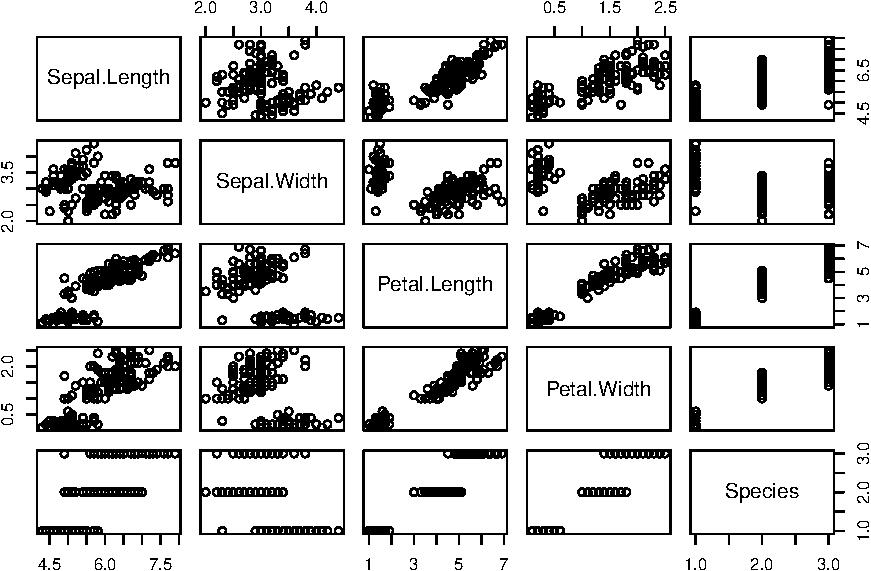
\includegraphics{00_thesis_files/figure-latex/sourcing-1.pdf}
\caption{\label{fig:sourcing}Example plot created in a scoured R script.}
\end{figure}

For more on the code chunk options/parameters see \href{https://bookdown.org/yihui/rmarkdown/r-code.html}{R Markdown Ch. 2.6}.
For example, the \texttt{echo\ =\ FALSE} parameter was removed in the second code chunk to print of the R code that
generated Figure \ref{fig:sourcing}.

\hypertarget{cross-referencing}{%
\subsection{Cross referencing}\label{cross-referencing}}

You can cross-reference sections, equations, figures, and tables etc., see \href{https://bookdown.org/yihui/bookdown/markdown-extensions-by-bookdown.html}{Bookdown Ch. 2.2} and \href{https://bookdown.org/yihui/bookdown/cross-references.html}{Ch. 2.6} for details.\\
For example, Section \ref{sec:background} or Figure \ref{fig:sourcing}.

\hypertarget{citation-and-references}{%
\subsection{Citation and References}\label{citation-and-references}}

We strongly recommend to use \href{https://www.zotero.org/}{Zotero} as Reference management software (with \href{https://retorque.re/zotero-better-bibtex/}{Better Bibtex} extension). It is free and open source and has a nice \href{https://rstudio.github.io/visual-markdown-editing/citations.html}{R Studio integration} (see also \url{https://github.com/crsh/citr} and \url{https://github.com/paleolimbot/rbbt}).

See \href{https://bookdown.org/yihui/bookdown/citations.html}{Bookdown Ch. 2.8} on how to cite references in R Markdown and
some general background.

\hypertarget{sec:background}{%
\section{Background}\label{sec:background}}

Here goes some background, for example references on R Markdown \citep{xie2018rmd} and Bookdown \citep{xie2016bookdown}.

\hypertarget{sec:experiments}{%
\section{Experiments}\label{sec:experiments}}

Here go some experiments, for example the average speed in the cars data set is 15.4.

You can also produce tables directly using R code:

\begin{longtable}[t]{rrrrl}
\caption{\label{tab:tables-mtcars}A simple table.}\\
\toprule
Sepal.Length & Sepal.Width & Petal.Length & Petal.Width & Species\\
\midrule
5.1 & 3.5 & 1.4 & 0.2 & setosa\\
4.9 & 3.0 & 1.4 & 0.2 & setosa\\
4.7 & 3.2 & 1.3 & 0.2 & setosa\\
4.6 & 3.1 & 1.5 & 0.2 & setosa\\
5.0 & 3.6 & 1.4 & 0.2 & setosa\\
\bottomrule
\end{longtable}

\hypertarget{sec:conclusion}{%
\section{Conclusion}\label{sec:conclusion}}

Seriously, think about writing your thesis using R Markdown!

\newpage

\pagenumbering{Roman}

\hypertarget{appendix-appendix}{%
\appendix}


\hypertarget{sec:appA}{%
\section{RStudio Options settings}\label{sec:appA}}

Change the RStudio default options as follows:

Global Options

\begin{itemize}
\tightlist
\item
  General

  \begin{itemize}
  \tightlist
  \item
    Basic

    \begin{itemize}
    \tightlist
    \item
      Restore .RData into workspace at startup: unckeck
    \item
      Save workspace to .RData on exit: Never
    \end{itemize}
  \end{itemize}
\item
  R Markdown

  \begin{itemize}
  \tightlist
  \item
    Basic

    \begin{itemize}
    \tightlist
    \item
      Evaluate chunks in directory: document
    \end{itemize}
  \item
    Citations (requires Better BibTex extension for Zotero)

    \begin{itemize}
    \tightlist
    \item
      Use Better BibTex for citation keys and BibTex export: check
    \end{itemize}
  \end{itemize}
\end{itemize}

\newpage

  \bibliography{references.bib}

\newpage

\section*{Declaration of authorship}
\thispagestyle{empty}
\vspace{-1cm}

\vspace{2cm} I hereby declare that the report submitted is my own unaided work. All direct or indirect sources used
are acknowledged as references. I am aware that the Thesis in digital form can be examined for the use of unauthorized
aid and in order to determine whether the report as a whole or parts incorporated in it may be deemed as plagiarism.
For the comparison of my work with existing sources I agree that it shall be entered in a database where it shall also
remain after examination, to enable comparison with future Theses submitted. Further rights of reproduction and usage,
however, are not granted here. This paper was not previously presented to another examination board and has not been
published.

\vspace{3cm}
\hfill\rule{6cm}{0.4pt}\\
\noindent Munich, \dueday~\duemonth~\dueyear \hfill \myname
\cleardoublepage

\end{document}
